%======================================================================
% 4. DETERMINISTIC AND ROBUST DESIGN FORMULATIONS
%======================================================================
\section{Deterministic and robust design formulations}
\label{sec:formulation}

Both formulations share the same design variables, constraints and
objectives; they differ only in how the uncertain inputs enter. Throughout,
$\mathbf{x}\in[0,1]^3$ denotes the normalized shape and
$\mathbf{z}=(\gamma_0,V_0,k_{CD},k_{CL})$ the uncertain inputs, with nominal
value $\mathbf{z}_0=(-2^\circ,7830\ \si{\metre\per\second},1,1)$.

\subsection{Deterministic baseline}
\label{sec:detform}

The deterministic problem is the formulation of the underlying thesis:
evaluate every objective and constraint at the nominal uncertain inputs,
\begin{equation}
\min_{\mathbf{x}\in[0,1]^3}\ \bigl(-\eta_V(\mathbf{x}),\;
  Q_s(\mathbf{x},\mathbf{z}_0),\; -sg(\mathbf{x},\mathbf{z}_0)\bigr),
\label{eq:det}
\end{equation}
subject to five constraints, written as $g_i\le 0$:
\begin{equation}
\frac{q_{\mathrm{stag}}^{\max}}{700\ \si{\kilo\watt\per\square\metre}}-1,\quad
\frac{q_{\mathrm{shldr}}^{\max}}{1000\ \si{\kilo\watt\per\square\metre}}-1,\quad
\frac{n_{\max}}{5\,g}-1,\quad
\left.\frac{\partial C_m}{\partial\alpha}\right|_{\mathrm{trim}},\quad
\alpha_{\mathrm{trim}}-\theta_{\mathrm{sp}} .
\label{eq:detcon}
\end{equation}
The first three bound peak heating and deceleration; the fourth enforces
static stability at trim ($\partial C_m/\partial\alpha\le0$, evaluated at
$M=10$); the fifth requires the trim angle of attack to fall on the
spherical nose section ($\alpha_{\mathrm{trim}}\le\theta_{\mathrm{sp}}$,
``on-nose trim''). The last two depend on $\mathbf{x}$ only. In this study
the deterministic problem is solved on the surrogate at $\mathbf{z}_0$;
nominal values quoted for specific designs come from the simulator itself.

\subsection{Robust moment formulation}
\label{sec:robform}

The robust formulation replaces each uncertain objective by its first two
moments under the uncertainty model and adds heat-load dispersion as an
explicit fourth objective,
\begin{equation}
\min_{\mathbf{x}\in[0,1]^3}\ \bigl(-\eta_V,\; \mathrm{E}[Q_s],\;
  -\mathrm{E}[sg],\; \sigma_{Q_s}\bigr),
\label{eq:rob}
\end{equation}
subject to the same geometry constraints and to moment versions of the three
peak constraints, in the spirit of feasibility-robustness formulations
\cite{du2000robust},
\begin{equation}
\mathrm{E}[g_i(\mathbf{x},\mathbf{z})] + 2\,\sigma_{g_i}(\mathbf{x})
  \;\le\; 0 , \qquad i=1,2,3 .
\label{eq:robcon}
\end{equation}
The $\mathrm{E}+2\sigma$ form is a deliberate choice: it keeps the moment
engine free of tail-quantile inversions, which Gaussian-process surrogates
support poorly in log space, and Section~\ref{sec:verification} checks the
implied exceedance probabilities directly by simulation. No distributional
claim is attached to the $2\sigma$ multiple --- under the skewed and
sometimes bimodal output distributions it is not a 95\% quantile; the
design contract is the inequality itself, and simulation shows what it
buys: every verified robust-front design met the constraints with zero
exceedances in 300 runs (rule-of-three upper bound $\approx$1\%), while
the point-feasible fragile deterministic design of
Section~\ref{sec:verification} exceeded the shoulder-heating limit in
9.7\% of runs. Exceedance
probabilities $P(q>\text{limit})$, computed from the lognormal predictive
distribution averaged over the uncertainty sample, are reported throughout
as audit quantities.

The dispersion objective uses a variance-inflated standard deviation,
\begin{equation}
\sigma_{Q_s}^{\,\mathrm{infl}} = \sqrt{
  \mathrm{E}_{\mathbf{z}}\!\left[\mathrm{Var}_{\mathrm{GP}}\right] +
  \mathrm{Var}_{\mathbf{z}}\!\left[\mathrm{E}_{\mathrm{GP}}\right]},
\label{eq:infl}
\end{equation}
the law of total variance applied to the surrogate prediction: the first
term is the mean surrogate (epistemic) variance over the uncertainty sample,
the second the physical (aleatory) variance of the surrogate mean. The
inflated form is used consistently for $\sigma_{Q_s}$ and for the
constraints of Eq.~\eqref{eq:robcon}. Its justification is empirical. A
probe of five designs spread over the design space, each propagated through
the true simulator with 60 uncertainty samples (Fig.~\ref{fig:probe}),
measured the true dispersion-to-surrogate-error ratio at 1.6--5.6 across
outputs: dispersion exceeds surrogate error everywhere, so the aleatory term
dominates and the inflation adds only 3--6\% to $\sigma_{Q_s}$ while
guarding against candidates whose surrogate error would otherwise be
invisible to the formulation.

One candidate constraint was deliberately dropped. The probability of the
slow, lofted family spans 0.34--0.59 over a 300-point scan of the whole
design space: it is set by the $\gamma_0$ dispersion, not by geometry, so a
constraint such as $P(\text{slow})\le0.05$ would be infeasible everywhere
and uninformative. $P(\text{slow})$ correlates with $\sigma_{Q_s}$
($r\approx0.74$) and with $\mathrm{E}[sg]$, so the dispersion objective
already prices lofting; $P(\text{slow})$ is reported as a diagnostic.

\subsection{Common-random-number moment engine}
\label{sec:engine}

Both the robust objectives of Eq.~\eqref{eq:rob} and the audit of the
deterministic front are evaluated by one moment engine. A single
Latin-hypercube sample of $\mathbf{z}$ (fixed seed) is shared by every
candidate, making moment estimates smooth functions of $\mathbf{x}$: this
common-random-number construction is what lets a genetic algorithm optimize
moments without the fitness noise of independent re-sampling, and it makes
the two fronts commensurable. The engine evaluates the surrogates'
predictive mean and variance at all sample points in one batched call,
forms the moments of Eq.~\eqref{eq:rob} and the inflated
variance of Eq.~\eqref{eq:infl}, and accumulates the lognormal-tail
exceedance probabilities; $\eta_V$ is exact geometry and the family and
capture classifiers supply $P(\text{slow})$ and $P(\text{capture})$. During
optimization a 500-point sample is used ($\approx$0.65~s per candidate);
every statistic reported in this paper is recomputed at $n_z=2000$.
All tables and figures regenerate from the frozen datasets with the
accompanying scripts, one command per artefact; the headline statistics
of Section~\ref{sec:matched} reproduce exactly from the saved fronts, as
does the baseline column of the sensitivity study.

\subsection{Optimizer setup and convergence}
\label{sec:optimizer}

Both formulations are solved with NSGA-II \cite{deb2002nsga2} via pymoo
\cite{blank2020pymoo}. The deterministic front uses a population of 200 for
300 generations; the robust front, whose evaluations are two orders of
magnitude dearer, uses 150 for 200 generations and was run once (about ten
hours); the deterministic run takes minutes and was repeated with three
seeds. Convergence and repeatability are documented rather than assumed
(Fig.~\ref{fig:convergence}): both fronts fill by generation 3--4 and the
design movement settles to $\varepsilon=6\times10^{-3}$--$10^{-2}$
thereafter; merging the three deterministic runs leaves 508 of 600 designs
non-dominated, with per-seed contributions of 166/167/175 and at most 14\%
cross-seed domination --- seed noise shifts front membership at the margins,
not the front itself. The robust front was repeated with two further
independent seeds: objective statistics coincide (median
$\mathrm{E}[sg]=5{,}212$--$5{,}405$~km; dispersion floor
16.36--\SI{16.4}{\mega\joule\per\square\metre}), the merged non-dominated
set of 450 designs retains 401 with balanced per-seed contributions
(135/127/139), and pairwise cross-domination is 3--10\% --- tighter than
the deterministic trio. Appendix~\ref{app:seeds} lists the full
comparison. The common-random-number engine additionally smooths
the robust fitness landscape.

\begin{figure}[htbp]
\centering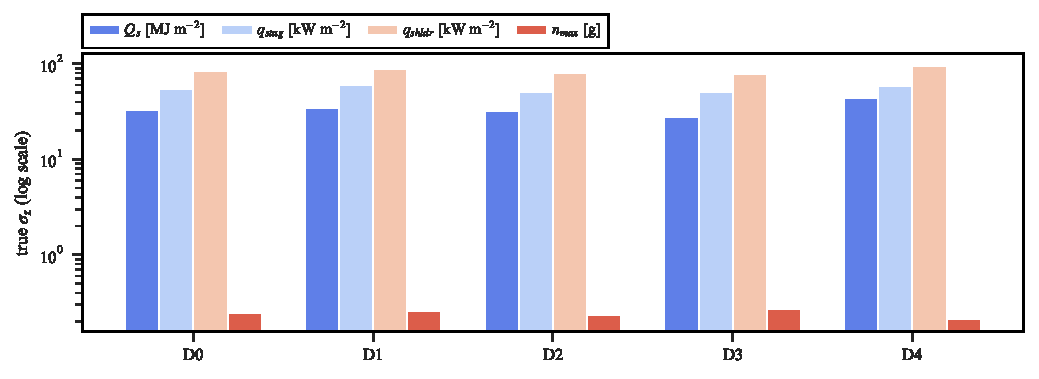
\includegraphics[width=\linewidth]{fig6_probe_true_sigma}
\caption{True uncertainty-driven dispersion $\sigma_z$ of the five probe
  designs ($5\times60$ simulator runs, $t_{\max}=\SI{14400}{\s}$) against
  the final-gate surrogate RMSE. Ratios $\sigma_z/\mathrm{RMSE}=1.6$--$5.6$
  justify the variance-inflated $\sigma_{Q_s}$ objective
  \eqref{eq:infl}.}
\label{fig:probe}
\end{figure}

\begin{figure}[htbp]
\centering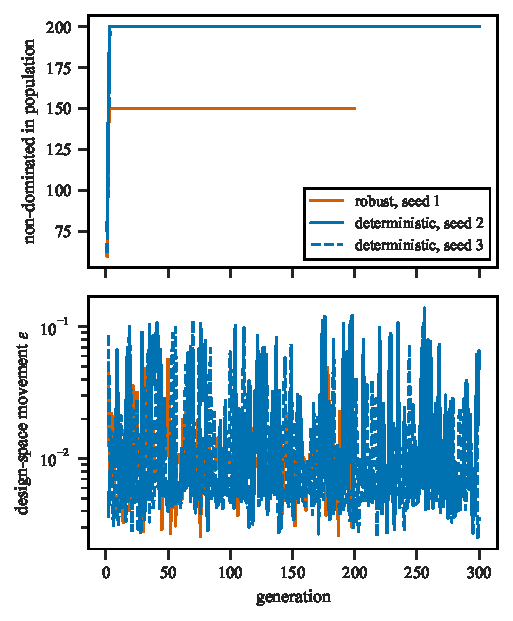
\includegraphics[width=\linewidth]{figS1_nsga2_convergence}
\caption{NSGA-II convergence evidence: per-generation non-dominated count
  and design-space movement ($\varepsilon$) for the robust run and two
  deterministic seeds. Fronts fill by generation 3--4; the movement decays
  to a recombination-noise floor of $6\times10^{-3}$--$10^{-2}$.}
\label{fig:convergence}
\end{figure}
